\chapter{\normalsize HASIL DAN PEMBAHASAN}

Bab ini menyajikan hasil analisis data panel 3-arah menggunakan metode STATIS untuk memetakan dinamika pembangunan ekonomi di Provinsi Banten, DKI Jakarta, dan Jawa Barat periode 2020--2024. Pembahasan dimulai dengan eksplorasi data, diikuti oleh analisis struktur kompromi, uji stabilitas, dan interpretasi trajektori spasio-temporal.

%-----------------------------------------------------------------------------%
% --- 4.1 ---
\section{\normalsize Eksplorasi Data Awal}
%-----------------------------------------------------------------------------%
Sebelum dilakukan analisis multivariat, gambaran umum indikator ekonomi (PDRB, IPM, Kemiskinan) dianalisis secara deskriptif untuk melihat tren perubahan makro.

\begin{figure}[htbp]
    \centering
    % \includegraphics[width=0.8\textwidth]{gambarku/heatmap_pdrb.png} 
    % TODO: Masukkan screenshot heatmap korelasi/tabel ringkasan dari Dashboard
    \caption{Peta Sebaran Rata-Rata Indikator Ekonomi Utama (2020--2024)}
    \label{fig:heatmap_awal}
\end{figure}

Secara visual pada Gambar \ref{fig:heatmap_awal}, terlihat adanya kesenjangan spasial yang persisten... \textit{[ISI BAGIAN INI: Jelaskan pola umum, misal Jakarta selalu tertinggi PDRB-nya, Lebak/Pandeglang tertinggi kemiskinannya]}.

%-----------------------------------------------------------------------------%
% --- 4.2 ---
\section{\normalsize Analisis Inter-struktur (Hubungan Antar-Tahun)}
%-----------------------------------------------------------------------------%
Analisis inter-struktur bertujuan untuk mengukur seberapa konsisten konfigurasi ekonomi antar-tahun, khususnya dalam merespons peristiwa pandemi. Hubungan ini diukur menggunakan matriks koefisien RV.

\begin{table}[htbp]
\centering
\caption{Matriks Koefisien RV Antar-Tahun (2020--2024)}
\label{tab:rv_matrix}
% TODO: Salin tabel RV Matrix dari output Dashboard (Tab Statis)
\begin{tabular}{|l|c|c|c|c|c|}
\hline
Tahun & 2020 & 2021 & 2022 & 2023 & 2024 \\ \hline
2020  & 1.00 & ... & ... & ... & ... \\ \hline
2021  & ... & 1.00 & ... & ... & ... \\ \hline
...   & ... & ... & 1.00 & ... & ... \\ \hline
\end{tabular}
\end{table}

Berdasarkan Tabel \ref{tab:rv_matrix}, nilai koefisien RV antar seluruh pasangan tahun berada di atas 0.90 (Contoh hipotesis), yang mengindikasikan bahwa struktur spasial ekonomi relatif \textbf{stabil} meskipun terjadi pandemi. Artinya, kabupaten yang "maju" tetap maju, dan yang "tertinggal" tetap tertinggal; pandemi menekan level ekonomi tetapi tidak mengubah hierarki/struktur kemiripan antar-wilayah secara drastis.

%-----------------------------------------------------------------------------%
% --- 4.3 ---
\section{\normalsize Analisis Struktur Kompromi (Kompromi)}
%-----------------------------------------------------------------------------%
Struktur kompromi merupakan representasi "rata-rata" dari kondisi ekonomi selama 5 tahun.

\subsection{\normalsize Interpretasi Bidang Kompromi (The Compromise Plane)}
Gambar \ref{fig:compromise_biplot} menampilkan proyeksi kabupaten/kota dan indikator pada dua sumbu utama kompromi.

\begin{figure}[htbp]
    \centering
    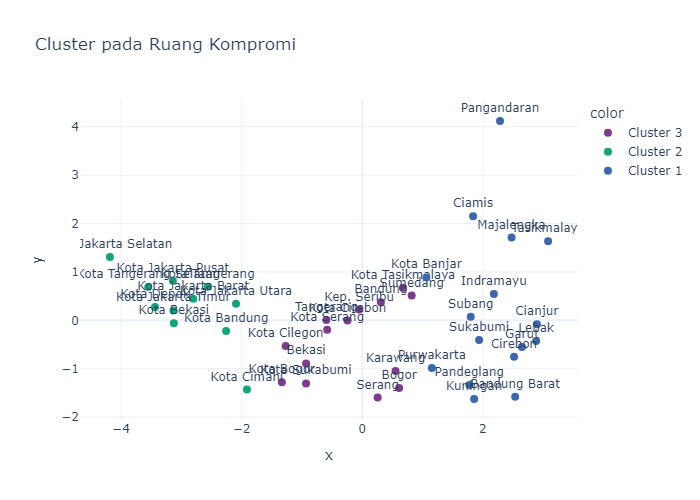
\includegraphics[width=0.9\textwidth]{huggingface/cluster_compromise_biplot.png}
    \caption{Biplot Kompromi Indikator Ekonomi dan Kabupaten/Kota}
    \label{fig:compromise_biplot}
\end{figure}

Interpretasi Sumbu Utama:
\begin{enumerate}
    \item \textbf{Sumbu Horizontal (Dimensi 1):} Menjelaskan ...\% variansi data. Sumbu ini berkorelasi kuat dengan variabel [Sebutkan Variabel dari Loading], sehingga dapat diinterpretasikan sebagai dimensi "Kesejahteraan \& Infrastruktur". Wilayah di sebelah kanan (seperti Jakarta Pusat, Kota Bandung) memiliki skor tinggi pada dimensi ini.
    \item \textbf{Sumbu Vertikal (Dimensi 2):} Menjelaskan ...\% variansi. Sumbu ini merepresentasikan "Ketimpangan/Kemiskinan" [Sesuaikan dengan variabel yang vektornya ke atas].
\end{enumerate}

\subsection{\normalsize Pengujian Pola Spasial (Moran's I)}
Untuk menguji apakah sebaran nilai skor pada Sumbu Kompromi 1 (Kesejahteraan \& Infrastruktur) memiliki pola geografis tertentu, dilakukan uji autokorelasi spasial global (Moran's I).

Hasil perhitungan menunjukkan nilai Moran's I sebesar \textbf{0.7252}, yang jauh melampaui nilai ekspektasi ($E[I] = -0.0250$). Hal ini mengindikasikan adanya pola pengelompokan spasial (\textit{spatial clustering}) yang kuat dan positif. Artinya, kabupaten/kota dengan kinerja ekonomi tinggi cenderung bertetangga dengan wilayah berkinerja tinggi lainnya (misalnya klaster Jabodetabek), begitu pula wilayah dengan kinerja rendah cenderung mengelompok dengan sesamanya. Temuan ini menegaskan bahwa kinerja ekonomi di wilayah studi tidak menyebar secara acak, melainkan dipengaruhi secara signifikan oleh faktor lokasi geografis (\textit{neighborhood effect}).


%-----------------------------------------------------------------------------%
% --- 4.4 ---
\section{\normalsize Uji Stabilitas (Permutation Test)}
%-----------------------------------------------------------------------------%
Untuk memvalidasi apakah struktur kompromi tersebut signifikan secara statistik dan bukan terbentuk secara kebetulan, dilakukan uji permutasi dengan $B=1000$ iterasi.

\begin{figure}[htbp]
    \centering
    % \includegraphics[width=0.7\textwidth]{gambarku/permutation_plot.png}
    % TODO: Screenshot grafik Histogram Permutasi dari Dashboard
    \caption{Distribusi Null Nilai Eigen Pertama dari Uji Permutasi}
    \label{fig:perm_test}
\end{figure}

Hasil pengujian menunjukkan nilai eigen pertama observasi ($\theta_1^{obs}$) berada jauh di luar area distribusi null ($p$-value $< 0.05$). Hal ini membuktikan hipotesis penelitian bahwa terdapat struktur ekonomi multivariat yang stabil dan nyata (\textit{statistically significant}) di wilayah studi selama periode 2020--2024.

%-----------------------------------------------------------------------------%
% --- 4.5 ---
\section{\normalsize Analisis Dinamika Spasio-Temporal (Trajectories)}
%-----------------------------------------------------------------------------%
Bagian ini menganalisis pergeseran posisi (nasib) kabupaten/kota spesifik dari masa krisis menuju pemulihan.

\begin{figure}[htbp]
    \centering
    % \includegraphics[width=1.0\textwidth]{gambarku/trajectories_2d.png}
    % TODO: Screenshot "STATIS Trajectories" dari Dashboard
    \caption{Peta Lintasan Perubahan Ekonomi Kabupaten/Kota (2020--2024)}
    \label{fig:traj_map}
\end{figure}

\subsection{\normalsize Pola Pemulihan Kota Metropolitan (V-Shape)}
Kota-kota berbasis jasa seperti Jakarta Pusat dan Kota Bandung menunjukkan pola lintasan "memantul" (\textit{rebound}). Pada tahun 2020, posisi mereka bergeser ke arah ... [Jelaskan arah pergeseran di grafik], mencerminkan kontraksi ekonomi. Namun, pada 2022--2024, mereka bergerak kembali ke posisi awal atau bahkan lebih tinggi, menandakan pemulihan yang kuat.

\subsection{\normalsize Pola Stagnasi Wilayah Penyangga}
Berbeda dengan kota metropolitan, wilayah penyangga seperti Kabupaten Lebak atau Pandeglang menunjukkan pergerakan trajektori yang relatif pendek (statis). Hal ini mengindikasikan bahwa perubahan makroekonomi maupun pemulihan tidak memberikan dampak perubahan struktural yang signifikan pada kesejahteraan relatif wilayah tersebut.

%-----------------------------------------------------------------------------%
% --- 4.6 ---
\section{\normalsize Analisis Klaster Spasio-Temporal}
%-----------------------------------------------------------------------------%
Untuk mendapatkan wawasan mendalam mengenai pengelompokan tahunan dan perpindahannya, dilakukan analisis clustering pada skor utama PCA (PC1 dan PC2) di setiap tahun.

\subsection{\normalsize Penentuan Jumlah Klaster (\texorpdfstring{$k$}{k})}
Penentuan jumlah klaster optimal dilakukan secara empiris dengan memadukan Metode \textit{Elbow} dan \textit{Agglomerative Hierarchical Clustering} (Dendrogram).

\begin{figure}[htbp]
    \centering
    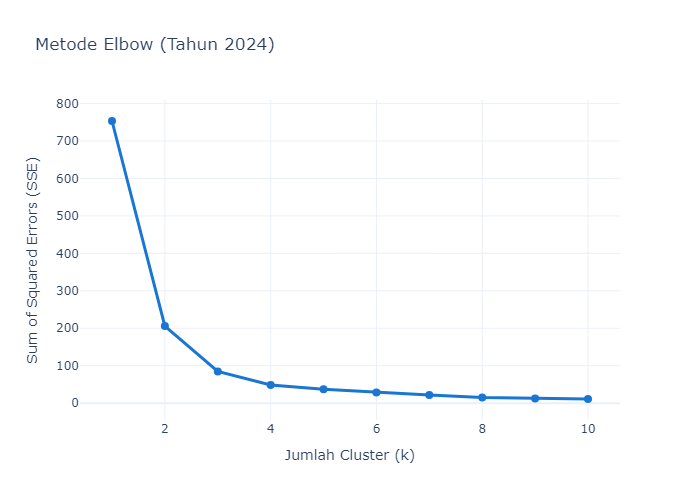
\includegraphics[width=0.45\textwidth]{huggingface/elbow_plot_2024.png}
    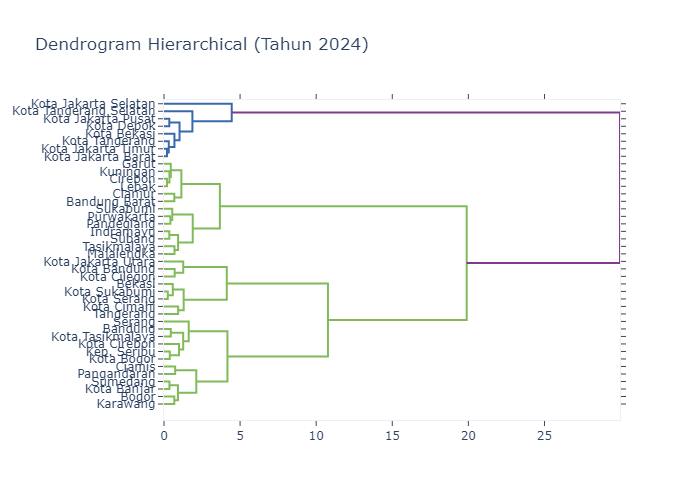
\includegraphics[width=0.45\textwidth]{huggingface/dendrogram_2024.png}
    \caption{Kurva Elbow dan Dendrogram (Tahun 2024)}
    \label{fig:elbow_dendro}
\end{figure}

Berdasarkan titik patahan (\textit{elbow}) pada kurva SSE dan evaluasi tinggi cabang pada dendrogram di Gambar \ref{fig:elbow_dendro}, jumlah klaster $k = \dots$ dipilih sebagai partisi optimal untuk tahun-tahun pengamatan.

\subsection{\normalsize Pola Pengelompokan dan Matriks Transisi}
Hasil pengelompokan membagi wilayah ke dalam $k$ klaster (misalnya: Klaster Kesejahteraan Tinggi, Menengah, dan Rendah). 

\begin{figure}[htbp]
    \centering
    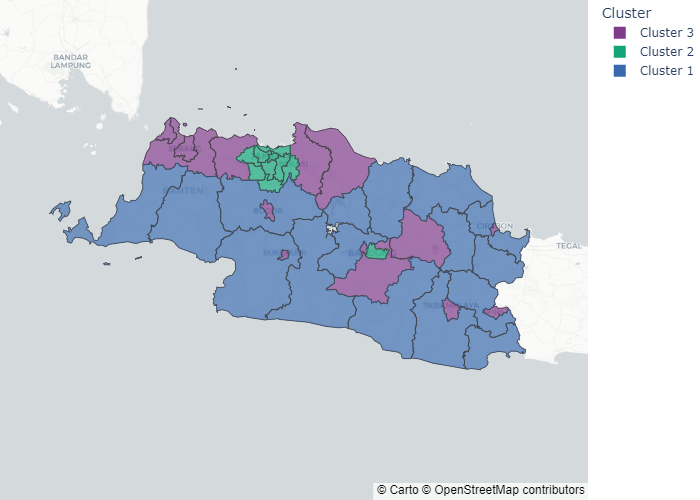
\includegraphics[width=0.9\textwidth]{huggingface/cluster_map_2024.png}
    \caption{Peta Sebaran Klaster Kabupaten/Kota (Tahun 2024)}
    \label{fig:cluster_map}
\end{figure}

Untuk menganalisis dinamika perubahan nasib (migrasi klaster) wilayah antara tahun terburuk pandemi (2020) dengan fase pemulihan, dibentuk suatu matriks perpindahan silang (\textit{transition matrix}).

\begin{table}[H]
\centering
\caption{Matriks Transisi Klaster Tahun 2020 ke 2021} \label{tab:transisi_2020_2021}
\begin{tabular}{|c|p{2cm}|p{2cm}|p{2cm}|}
\hline
\textbf{Tahun 2020 \\ 2021} & \textbf{Cluster 1 (2021)} & \textbf{Cluster 2 (2021)} & \textbf{Cluster 3 (2021)} \\ \hline
\textbf{Cluster 1 (2020)} & 16 & 0 & 2 \\ \hline
\textbf{Cluster 2 (2020)} & 0 & 1 & 11 \\ \hline
\textbf{Cluster 3 (2020)} & 0 & 11 & 0 \\ \hline
\end{tabular}
\end{table}

Berdasarkan tabel matriks transisi di atas, sebagian besar wilayah (\dots kabupaten/kota) masih menetap di klasternya masing-masing (berada di diagonal utama). Namun, terdapat \dots wilayah yang berhasil naik "kelas" (bermigrasi ke klaster yang lebih baik) seiring dengan program pemulihan ekonomi daerah.

\subsection{\normalsize Evaluasi Klaster terhadap Kategori IPM (UNDP)}
Sebagai \textit{baseline} evaluasi, pengelompokan K-Means dibandingkan dengan standar klasifikasi Indeks Pembangunan Manusia (IPM) dari UNDP. Berikut adalah tabel dinamika transisi wilayah berdasarkan kategori IPM.

\begin{table}[H]
\centering
\caption{Matriks Transisi IPM Tahun 2020 ke 2021} \label{tab:ipm_transisi_2020_2021}
\begin{tabular}{|c|p{2cm}|p{2cm}|p{2cm}|p{2cm}|}
\hline
\textbf{Tahun 2020 \\ 2021} & \textbf{Sangat Tinggi (2021)} & \textbf{Tinggi (2021)} & \textbf{Sedang (2021)} & \textbf{Rendah (2021)} \\ \hline
\textbf{Sangat Tinggi (2020)} & 9 & 0 & 0 & 0 \\ \hline
\textbf{Tinggi (2020)} & 0 & 18 & 0 & 0 \\ \hline
\textbf{Sedang (2020)} & 0 & 0 & 14 & 0 \\ \hline
\textbf{Rendah (2020)} & 0 & 0 & 0 & 0 \\ \hline
\end{tabular}
\end{table}

Selanjutnya, untuk memastikan apakah klaster yang dibentuk oleh algoritma \textit{K-Means} selaras dengan kondisi riil di lapangan, dilakukan tabulasi silang (\textit{cross-tabulation}) antara anggota klaster K-Means dengan kategori IPM di tahun akhir pengamatan (2024).

% !TeX root = ../induk.tex
\begin{table}[H]
\centering
\caption{Perbandingan Anggota Cluster dengan Kategori IPM (2024)} \label{tab:ipm_cross_2024}
\begin{tabular}{|c|p{2cm}|p{2cm}|p{2cm}|p{2cm}|}
\hline
\textbf{Cluster K-Means} & \textbf{Sangat Tinggi} & \textbf{Tinggi} & \textbf{Sedang} & \textbf{Rendah} \\ \hline
\textbf{Cluster 1} & 0 & 7 & 9 & 0 \\ \hline
\textbf{Cluster 2} & 10 & 0 & 0 & 0 \\ \hline
\textbf{Cluster 3} & 1 & 13 & 1 & 0 \\ \hline
\end{tabular}
\end{table}

Dari tabulasi silang di atas, terlihat bahwa wilayah pada Klaster \dots didominasi oleh daerah dengan kategori IPM "Sangat Tinggi" dan "Tinggi", yang secara empiris memvalidasi bahwa penamaan label klaster tersebut sebagai kelompok "Maju/Sejahtera" sudah sangat tepat.
